\documentclass[preview,border=10pt]{standalone}

\usepackage[utf8]{inputenc}				% Кодировка utf8
\usepackage[english, russian]{babel}	% Языки: русский, английский
\usepackage{amssymb,amsmath}

\usepackage{graphicx}
\usepackage[noend]{algpseudocode}

\DeclareMathOperator*{\argmax}{arg\,max}
\DeclareMathOperator*{\argmin}{arg\,min}
\renewcommand{\algorithmiccomment}[1]{{\quad\footnotesize // #1}}

\begin{document}
	\begin{center}
		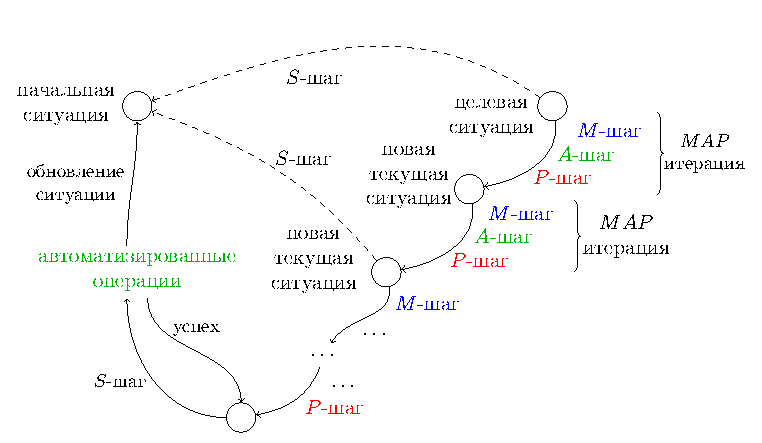
\includegraphics[width=\textwidth]{../images/algo/ru/beh_plan2_ru}
	\end{center}
	
	Алгоритм процесса планирования поведения в знаковой картине мира.
	
	\textbf{Алгоритм MAP-planner}
	\vspace*{2pt}
	\hrule
	\vspace*{1pt}
	\hrule
		
	\begin{algorithmic}[1]
			\Require начальная ситуация $S_{st}$, целевая ситуация $S_{goal}$, включающая в себя знак мотива $s_{goal}$, функции оценки $\Phi_a$ и $\Phi_p$;
	\Ensure план $Plan$;
	\algrule
	\State $F_{st}^{obj}=\varnothing$; \Comment{множество объектных признаков начальной ситуации}
	\ForAll $s\in S_{st}$
		\If{$f(s)\in\mathcal F^{obj}$}
			\State $F_{st}^{obj}= F_{st}^{obj}\cup\{f(s)\}$; 
		\EndIf
	\EndFor
	
	\State $Plan=\Call{Planning}{\varnothing,S_{goal}}$;
	
	\Function{Planning}{$Plan, S_{cur}$}
		\State $F_{cur}=\bigcup\limits_{s\in S_{cur}}\{f(s)\}$; \Comment{множество признаков текущей ситуации планирования}
		\State $F_{st}=\bigcup\limits_{s\in S_{st}}\{f(s)\}$; \Comment{множество признаков начальной ситуации}
		\State $M_{st}=\bigcup\limits_{f\in F_{st}}m(f)$;
		\State $\Delta=F_{st}\setminus F_{cur}$; \Comment{текущая невязка состояний}
		
		\State $M_{forw}\subseteq M_{st}:\begin{cases}
			|\bigcup\limits_{\mu\in M_{forw}}F_A(\mu)\setminus\Delta|\rightarrow\max,\\
			|\bigcap\limits_{\mu\in M_{forw}}F_A(\mu)\setminus\Delta|\rightarrow\min;
		\end{cases}$ \Comment{Решение minmax задачи}
		
		\ForAll $\mu_j\in M_{forw}$
			\If{$\exists \mu_k\in M_{forw}$ такой, что $\mu_k\not =\mu_i$ и $\mu_k$ конфликтует с $\mu_j$}
				\State $\mu_{del}=\argmin\limits_{\mu\in\{\mu_k,\mu_j\}}|F_A(\mu)\setminus\Delta|$;
				\State $M_{forw}= M_{forw}\setminus\{\mu_{del}\}$; \Comment{Удаляем конфликтующие признаки}
			\EndIf
		\EndFor
		
		\State $A_{forw} = \bigcup\limits_{\mu\in M_{forw}}\{\Call{Interior}{\mu}\}$; \Comment{текущее множестов личностных смыслов}
		\State $\tilde A_{forw}=\Phi_a(A_{forw},f_{goal})$; \Comment{выбор предпочитаемых действий}
		\If{$\bigcup\limits_{a\in \tilde A_{forw}}F_C(a)\subseteq F_{st}$ и $F_{cur}\subseteq F_{st}\cup\bigcup\limits_{a\in \tilde A_{forw}}F_C(a)\setminus\bigcup\limits_{a\in \tilde A_{forw}}F_D(a)$}
			\State \Return $Plan\cup{\tilde A_{forw}}$;		\Comment{возвращаем обновленный план}
		\Else
			\State $\Delta^* = \Phi_p(\Delta, f_{goal})$; \Comment{Ранжирование критических признаков}
			\State $\tilde F_a^{back} = \varnothing$; 
			\ForAll $f_k\in\Delta^*$ 
				\State $m_k = \tilde m(f_k)$; \Comment{определение значение $k$-го знака}
				\State $F_a^{back} = \varnothing$;
				\ForAll $f_p\in m_k$
					\State $F_a^{back}=F_a^{back}\cup\{\Call{Interior}{f_p}\}$;
				\EndFor 
				\State $\tilde F_a^{back}=\tilde F_a^{back}\cup\Phi_a(F_a^{back}, f_{goal})$; \Comment{выбор предпочитаемых действий}
			\EndFor
			
			\ForAll $f_j\in \tilde F_a^{back}$
				\If{$\exists f_k\in \tilde F_a^{back}$ такой, что $f_k\not =f_i$ и $f_k$ конфликтует с $f_j$}
					\State $\tilde F_a^{back} = \tilde F_a^{back}\setminus\{f_k\}$; \Comment{Удаляем конфликтующие признаки}
				\EndIf
			\EndFor
			
			
			\If{$\Delta\not\subseteq\bigcup\limits_{f\in\tilde F_a^{back}}F_A(f)$}
				\State\Return невозможно построить план;
			\Else
				\State \Return \Call{Planning}{$Plan, \bigcup\limits_{f\in F_a^{back}}F_C(f)$};						
			\EndIf
		\EndIf

	\EndFunction
	\end{algorithmic}

\end{document}
